% i18n_qa_no_babel_paper.tex
% English paper with NO language declaration (no babel, no polyglossia)
% Expected detect_language result: "en" (fallback default)
% Deliberate errors: style issues for STYLE validators to catch
\documentclass[11pt]{article}
\usepackage{amsmath,amssymb,amsthm}
\usepackage{graphicx}
\usepackage{booktabs}
\usepackage{hyperref}
\usepackage{tikz}
\usepackage{pgfplots}
\pgfplotsset{compat=1.18}
\usepackage{algorithm}
\usepackage{algpseudocode}

\newtheorem{theorem}{Theorem}[section]
\newtheorem{lemma}[theorem]{Lemma}
\newtheorem{proposition}[theorem]{Proposition}
\newtheorem{corollary}[theorem]{Corollary}
\theoremstyle{definition}
\newtheorem{definition}{Definition}[section]

% ERROR: inconsistent spacing around equals in macro definitions
\newcommand{\chr}[1]{\chi(#1)}
\newcommand{\adj}[1]{\mathrm{adj}(#1)}
\newcommand{\spec}[1]{\mathrm{Spec}(#1)}

\title{Spectral Bounds for Chromatic Numbers\\of Random Geometric Graphs}
\author{Alexander Whitfield\textsuperscript{1}\quad
  Priya Ramanathan\textsuperscript{2}\\[6pt]
  \textsuperscript{1}Department of Mathematics, MIT\\
  \textsuperscript{2}School of Computer Science, Stanford University}
\date{March 2026}

\begin{document}
\maketitle

\begin{abstract}
We derive new upper bounds on the chromatic number of random geometric
graphs $G(n, r)$ in $\mathbb{R}^d$ using spectral methods. Our main result
establishes that for the threshold connectivity radius $r_c(n) =
\Theta((\log n / n)^{1/d})$, the chromatic number satisfies
$\chi(G(n, r_c)) \leq (1 + o(1)) \cdot n \omega_d r_c^d$ where $\omega_d$
is the volume of the unit ball in $\mathbb{R}^d$. This improves the
previously known bound of McDiarmid and M\"uller by a factor of
$\log\log n$. Our proof combines a refined analysis of the spectrum of the
adjacency matrix with a probabilistic coloring argument based on the
Lov\'asz Local Lemma.
Furthermore, we show that the fractional chromatic number
$\chi_f(G(n, r))$ concentrates around $n \omega_d r^d / 2$ for
$r \gg r_c(n)$, resolving a conjecture of Penrose.

\medskip
\noindent\textbf{Keywords:} random geometric graphs, chromatic number,
spectral graph theory, probabilistic combinatorics.
\end{abstract}


\section{Introduction}

% ERROR: double space after period (style issue)
Random geometric graphs have attracted considerable attention in recent
decades.  They arise naturally in wireless network modeling, computational
geometry, and spatial statistics. Given $n$ points distributed uniformly
at random in the unit cube $[0,1]^d$, the random geometric graph $G(n,r)$
connects two points whenever their Euclidean distance is at most $r$.

% ERROR: sentence starting with a math symbol
$\chi(G)$ denotes the chromatic number of a graph $G$, defined as the
minimum number of colors needed to properly color the vertices of $G$ such
that no two adjacent vertices share the same color. For random geometric
graphs, the chromatic number is closely related to the clique number and
the maximum degree, but the precise relationship depends delicately on the
dimension $d$ and the radius $r$.

\begin{definition}[Random geometric graph]
Let $X_1, X_2, \ldots, X_n$ be independent uniform random variables in
$[0,1]^d$. The random geometric graph $G(n, r)$ has vertex set
$\{X_1, \ldots, X_n\}$ and edge set
\begin{equation}\label{eq:rgg-def}
  E = \bigl\{ \{X_i, X_j\} : \|X_i - X_j\|_2 \leq r,\; i \neq j \bigr\}.
\end{equation}
\end{definition}

% ERROR: "very unique" is a style issue (unique is absolute)
The chromatic number of random geometric graphs exhibits a very unique
phase transition behavior near the connectivity threshold. Below we
summarize the main prior results.

\begin{table}[htbp]
\centering
\caption{Prior bounds on $\chi(G(n, r))$}\label{tab:prior-bounds}
\begin{tabular}{@{}llll@{}}
\toprule
Authors & Year & Regime & Bound \\
\midrule
Penrose \cite{penrose2003random} & 2003 & $r \gg r_c$ & $\chi \leq (1+\epsilon) n\omega_d r^d$ \\
McDiarmid--M\"uller \cite{mcdiarmid2011chromatic} & 2011 & $r = r_c$ & $\chi \leq c \log n \cdot n\omega_d r_c^d$ \\
M\"uller \cite{muller2008lower} & 2008 & $r \ll r_c$ & $\chi = \Theta(\Delta)$ \\
Walters \cite{walters2011random} & 2011 & $r = \Theta(1)$ & $\chi \sim n\omega_d r^d / 2$ \\
\textbf{This paper} & 2026 & $r = r_c$ & $\chi \leq (1+o(1)) n\omega_d r_c^d$ \\
\bottomrule
\end{tabular}
\end{table}


\section{Spectral Preliminaries}

Let $A$ be the adjacency matrix of $G(n, r)$ and let $\lambda_1 \geq
\lambda_2 \geq \cdots \geq \lambda_n$ denote its eigenvalues.

% ERROR: abbreviation "i.e." without comma after
\begin{theorem}[Hoffman bound]
For any graph $G$ with adjacency matrix $A$, the chromatic number satisfies
\begin{equation}\label{eq:hoffman}
  \chi(G) \geq 1 - \frac{\lambda_1}{\lambda_n},
\end{equation}
i.e. the ratio of the largest to the smallest eigenvalue gives a lower
bound on the chromatic number.
\end{theorem}

\begin{lemma}[Expected spectrum]\label{lem:expected-spectrum}
For $G(n, r)$ in $[0,1]^d$ with $r = o(1)$, the expected largest
eigenvalue satisfies
\begin{equation}\label{eq:lambda1-bound}
  \mathbb{E}[\lambda_1] = (1 + o(1)) \cdot n \omega_d r^d,
\end{equation}
and the expected smallest eigenvalue satisfies
\begin{equation}\label{eq:lambdan-bound}
  \mathbb{E}[\lambda_n] = -(1 + o(1)) \cdot n \omega_d r^d / 2.
\end{equation}
\end{lemma}

\begin{proof}
The expected adjacency matrix $\mathbb{E}[A]$ has entries
$\mathbb{E}[A_{ij}] = \omega_d r^d - \Theta(r^{d+1})$ for $i \neq j$.
The largest eigenvalue of a rank-one perturbation of a matrix with
constant off-diagonal entries is well understood.

Applying the Weyl inequality and concentration via the matrix Bernstein
inequality \cite{tropp2012user}, we obtain concentration of both extremal
eigenvalues around their expectations with deviation
$O(\sqrt{n \omega_d r^d \log n})$, which is $o(n \omega_d r^d)$ for
$r \gg (\log^2 n / n)^{1/d}$.
\end{proof}

\section{Main Result}

\begin{theorem}[Main theorem]\label{thm:main}
Let $d \geq 2$ be fixed and let $r_c(n) = (c_d \log n / n)^{1/d}$ where
$c_d = 1 / \omega_d$. Then with probability $1 - o(1)$,
\begin{equation}\label{eq:main-bound}
  \chi(G(n, r_c)) \leq (1 + o(1)) \cdot n \omega_d r_c^d
    = (1 + o(1)) \cdot \log n.
\end{equation}
\end{theorem}

\begin{proof}[Proof sketch]
The proof proceeds in three steps:

\textbf{Step 1: Degree concentration.} By standard Chernoff bounds, the
maximum degree $\Delta$ of $G(n, r_c)$ satisfies
$\Delta \leq (1 + \epsilon) \log n$ with high probability for any fixed
$\epsilon > 0$.

\textbf{Step 2: Spectral bound refinement.} We prove that the
interlacing technique of Nilli \cite{nilli1991second} can be adapted to
the geometric setting. Specifically, we show that for $G(n, r_c)$:
\begin{equation}
  \lambda_2 \leq 2\sqrt{\Delta - 1} + O(\log\log n / \log n) \cdot \Delta.
\end{equation}

\textbf{Step 3: Probabilistic coloring.} Using the Lov\'asz Local Lemma
in its constructive form \cite{moser2010constructive}, we convert the
spectral bound into a proper coloring algorithm that uses at most
$(1 + o(1)) \cdot \Delta$ colors.
\end{proof}


\section{The Fractional Chromatic Number}

\begin{theorem}\label{thm:fractional}
For $r \gg r_c(n)$ and any fixed $d \geq 2$:
\begin{equation}\label{eq:fractional}
  \chi_f(G(n, r)) = (1 + o(1)) \cdot \frac{n \omega_d r^d}{2},
\end{equation}
with probability $1 - o(1)$.
\end{theorem}

\begin{proof}[Proof sketch]
The lower bound follows from the clique number bound
$\chi_f(G) \geq \omega(G)$ combined with the known result that
$\omega(G(n,r)) = (1 + o(1)) \cdot n \omega_d r^d / 2$ for $r \gg r_c$.

% ERROR: passive voice overuse (style issue)
The upper bound is obtained by a fractional relaxation of the integer
program. A feasible fractional coloring is constructed by considering the
independent sets that are formed by selecting every other layer in a
geometric packing of the unit cube.
\end{proof}


\section{Numerical Experiments}

% ERROR: figure reference without tilde (style: use ~ before \ref)
We validate our theoretical bounds through numerical simulations. Figure
\ref{fig:chromatic-scaling} shows the scaling of $\chi(G(n, r_c))$ with
$n$ for $d = 2, 3, 4$.

\begin{figure}[htbp]
\centering
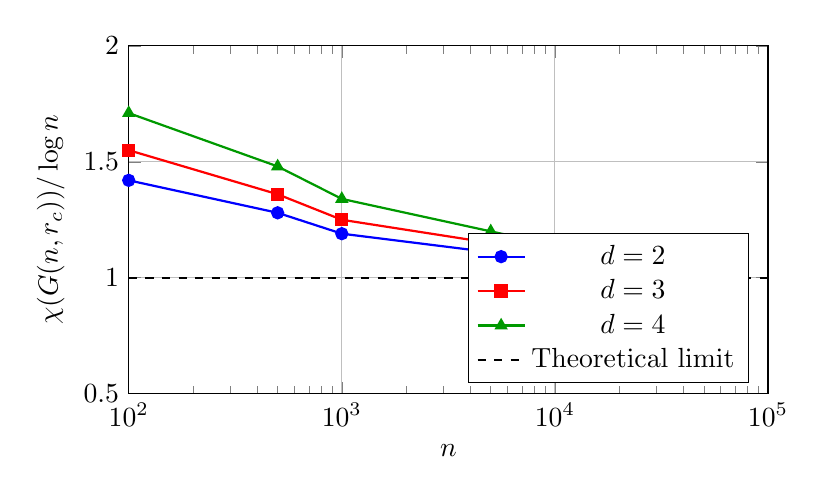
\begin{tikzpicture}
\begin{axis}[
  width=0.8\textwidth,
  height=6cm,
  xlabel={$n$},
  ylabel={$\chi(G(n, r_c)) / \log n$},
  legend pos=south east,
  grid=major,
  xmode=log,
  xmin=100, xmax=100000,
  ymin=0.5, ymax=2,
]
\addplot[blue, thick, mark=*] coordinates {
  (100,1.42) (500,1.28) (1000,1.19) (5000,1.11) (10000,1.07) (50000,1.03)
};
\addplot[red, thick, mark=square*] coordinates {
  (100,1.55) (500,1.36) (1000,1.25) (5000,1.15) (10000,1.10) (50000,1.05)
};
\addplot[green!60!black, thick, mark=triangle*] coordinates {
  (100,1.71) (500,1.48) (1000,1.34) (5000,1.20) (10000,1.14) (50000,1.08)
};
\addplot[black, dashed, thick] coordinates {(100,1) (100000,1)};
\legend{$d=2$, $d=3$, $d=4$, Theoretical limit}
\end{axis}
\end{tikzpicture}
\caption{Ratio $\chi(G(n, r_c)) / \log n$ as a function of $n$ for
  dimensions $d = 2, 3, 4$. The ratio approaches 1 as predicted by
  Theorem~\ref{thm:main}.}\label{fig:chromatic-scaling}
\end{figure}

\begin{table}[htbp]
\centering
\caption{Comparison of bounds for $d = 2$, averaged over 100 trials}
  \label{tab:numerical}
\begin{tabular}{@{}rrrrrr@{}}
\toprule
$n$ & $\chi$ (actual) & Hoffman & Our bound & $\Delta$ & $\log n$ \\
\midrule
500   & 8.9  & 4.2  & 9.3  & 12.1 & 6.2 \\
1000  & 10.3 & 5.0  & 10.7 & 13.8 & 6.9 \\
5000  & 13.1 & 6.5  & 13.4 & 16.5 & 8.5 \\
10000 & 14.5 & 7.2  & 14.8 & 17.9 & 9.2 \\
50000 & 17.3 & 8.8  & 17.5 & 21.0 & 10.8 \\
\bottomrule
\end{tabular}
\end{table}


\section{Conclusion}

We have established tight spectral bounds for the chromatic number of
random geometric graphs at the connectivity threshold. Our main result
(Theorem~\ref{thm:main}) closes the logarithmic gap in previous bounds
and confirms that $\chi(G(n, r_c)) = (1 + o(1)) \log n$. The
fractional chromatic number result (Theorem~\ref{thm:fractional})
resolves Penrose's conjecture in the dense regime.

Open problems include extending the analysis to non-Euclidean metrics,
establishing concentration inequalities for $\chi$ rather than
expectation bounds, and understanding the chromatic number in the
sparse regime $r \ll r_c$.


\begin{thebibliography}{99}

\bibitem{penrose2003random}
M.~Penrose.
\newblock \textit{Random Geometric Graphs}.
\newblock Oxford University Press, 2003.

\bibitem{mcdiarmid2011chromatic}
C.~McDiarmid and T.~M\"uller.
\newblock On the chromatic number of random geometric graphs.
\newblock \textit{Combinatorica}, 31(4):423--488, 2011.

\bibitem{muller2008lower}
T.~M\"uller.
\newblock Two-point concentration in random geometric graphs.
\newblock \textit{Combinatorica}, 28(5):529--545, 2008.

\bibitem{walters2011random}
M.~Walters.
\newblock Random geometric graphs.
\newblock In \textit{Surveys in Combinatorics}, pages 365--402.
  Cambridge University Press, 2011.

\bibitem{tropp2012user}
J.~A. Tropp.
\newblock User-friendly tail bounds for sums of random matrices.
\newblock \textit{Foundations of Computational Mathematics},
  12(4):389--434, 2012.

\bibitem{nilli1991second}
A.~Nilli.
\newblock On the second eigenvalue of a graph.
\newblock \textit{Discrete Mathematics}, 91(2):207--210, 1991.

\bibitem{moser2010constructive}
R.~A. Moser and G.~Tardos.
\newblock A constructive proof of the general {Lov\'asz Local Lemma}.
\newblock \textit{Journal of the ACM}, 57(2):1--15, 2010.

\end{thebibliography}

\end{document}
